\documentclass[a4paper, 12pt, twoside, openright, fleqn]{book}

% language settings
\usepackage[italian]{babel}
\usepackage[T1]{fontenc}
\usepackage[utf8]{inputenc}
\usepackage{fancyhdr}
\usepackage{subcaption}
\usepackage[usenames, dvipsnames, table, tikz]{xcolor}
\usepackage{tikz,float,pdfpages,pgfplots,listing}
\usepackage{graphicx,graphics,wrapfig,changepage}

% math package
\usepackage{mathtools,amsthm,environ,cancel,cases}
\usepackage{amsmath, amssymb, dsfont, bm,blkarray}
\graphicspath{{./img/} {./.tmp/} }
% tikz figures
% \usepackage{tikz}
\usetikzlibrary{shapes, arrows, automata}
\usepackage{steinmetz}

% add support for url and cross-references in PDF output
\usepackage{url}
\renewcommand{\UrlFont}{\color{black}\small\ttfamily}
\usepackage[colorlinks=true, linkcolor=black, citecolor=black, urlcolor=black]{hyperref}

% support for glossary and acronyms
\usepackage[acronym]{glossaries}
% \newacronym{geraf}{GeRaF}{Geographic Random Forwarding}
% Costumization of theorem style
\newtheoremstyle{theoremdd}% name of the style to be used
  {\topsep}% measure of space to leave above the theorem. E.g.: 3pt
  {\topsep}% measure of space to leave below the theorem. E.g.: 3pt
  {\itshape}% name of font to use in the body of the theorem
  {0pt}% measure of space to indent
  {\bfseries}% name of head font %\color{Mahogany}
  { -- }% punctuation between head and body
  { }% space after theorem head; " " = normal interword space
  {\thmname{#1}\thmnumber{ #2}\thmnote{ (#3)}}

\theoremstyle{theoremdd}
% support for counting
\newtheorem{theorem}{Theorem}[section]
\newtheorem{corollary}{Corollary}[theorem]
\newtheorem{lemma}[theorem]{Lemma}
\newtheorem{definition}{Definition}
\newtheorem{remark}{Remark}
\newtheorem{example}{Example}

% added support for proof parts
\theoremstyle{remark}
\newtheorem{proofpart}{Part}
\renewcommand\theproofpart{\Roman{proofpart}}
\makeatletter
\@addtoreset{proofpart}{theorem}
\makeatother

% specific modification to basic book template of our book document
% \renewcommand{\chaptername}{Section}
% \addto\captionsenglish{\renewcommand{\chaptername}{Section}}

% \renewcommand\qedsymbol{\includegraphics[width=1.5cm]{occhiali}}
%\renewcommand\qedsymbol{$\square$\itshape QED}

%split and equation environment
\NewEnviron{esp}{%
\begin{equation}\begin{split}
  \BODY
\end{split}\end{equation}
}

\NewEnviron{esp*}{%
\begin{equation*}\begin{split}
  \BODY
\end{split}\end{equation*}
}


%------------------------------ define Abstract environment, missing in the 'book' class
\newenvironment{abstract}{\cleardoublepage \null \vfill \begin{center}\bfseries\abstractname \end{center}}{\vfill\null}
\addto\captionsenglish{\renewcommand*\abstractname{Sommario}} % change Abstract title
%------------------------------ active url
\usepackage{url}
%\usepackage{svg}
\usepackage{ifluatex}
\renewcommand{\UrlFont}{\color{black}\small\ttfamily}

% \usepackage[colorlinks=true, linkcolor=black, citecolor=black, urlcolor=black]{hyperref} % active ref

%------------------------------ macros
\newcommand{\sectionname}{Section} % define Section ref
\newcommand{\subsectionname}{Sub-section} % define Sub-section ref
\renewcommand*\arraystretch{1.4} % tables padding
\newcommand{\N}{\mathbb{N}}
\DeclareInputText{176}{°}

% Useful Aliases
\def\beq{\begin{equation}}
\def\eeq{\end{equation}}
\def\bal{\begin{align}}
\def\eal{\end{align}}
\def\prob{\ensuremath\mathbb{P}}
\def\exp{\ensuremath\mathbb{E}}
\def\pois{\mathcal P}
\newcommand{\Hb}{\mathbb{H}}
\newcommand{\Sb}{\mathbb{\Sigma}}
\newcommand{\U}{\mathbb{U}}
\newcommand{\F}{\mathbb{F}}
\newcommand{\V}{\mathbb{V}}
\newcommand{\A}{\mathbb{A}}
\newcommand{\B}{\mathbb{B}}
\newcommand{\C}{\mathbb{C}}
\newcommand{\E}{\mathbb{E}}
\newcommand{\I}{\mathbb{I}}
\newcommand{\Y}{\mathbb{Y}}
%\newcommand{\N}{\mathbb{N}}
\newcommand{\W}{\mathbb{W}}
\newcommand{\Z}{\mathbb{Z}}
\newcommand{\R}{\mathbb{R}}
\newcommand{\X}{\mathbb{X}}
\newcommand{\Pb}{\mathbb{P}}
\newcommand{\Q}{\mathbb{Q}}
\newcommand{\D}{\mathbb{D}}
\newcommand{\Rm}{\mathbb{R^{-1}}}
\newcommand{\J}{\mathbb{J}}
\newcommand*{\Chi}{\mbox{\Large $\chi$}}% big chi
\newcommand{\Fig}[1]{Fig.~\ref{#1}}
\newcommand{\eq}[1]{(\ref{#1})}
\newcommand{\Tab}[1]{Tab.~\ref{#1}}
\newcommand{\Sec}[1]{Sec.~\ref{#1}}
\newcommand{\indep}{\mathrel{\perp\mspace{-10mu}\perp}}
\newcommand{\RN}[1]{ \textup{\uppercase\expandafter{\romannumeral#1}}} %This is for inserting Roman Numbers (useful for \stackrel in equations so that you don't confuse indicating numbers from equation numbers

\begin{document}
\frontmatter

\begin{titlepage} %------------------------------ TITLE PAGE
\begin{center}

\hspace{0.5cm}

\emph{\Large{TELECOMMUNICATION NETWORKS}} \\
\vspace{1cm}
% \includegraphics[width=9cm]{img/bella.png}\\
\vspace{0.5cm}
{written with foolness by\par}
{\Large Matilde Boschiero\par}
\end{center}

\vfill
\begin{center}
\noindent\makebox[\linewidth]{\rule{\textwidth}{0.4pt}}
\textsc{Academic Year 2017/2018}
\end{center}
\end{titlepage}

\begingroup %------------------------------ CONTENTS
  \makeatletter
  \let\ps@plain\ps@empty
  \makeatother
  \tableofcontents
  \clearpage
\endgroup
\mainmatter
\chapter{Internet}
The Internet is a global system of interconnected computer networks that use the standard \textit{Internet
Protocol Suite (TCP/IP)} to serve several billion users worldwide. We can refer to it as a \textit{Network of Networks}.
\section{Overview}
\begin{itemize}
\item 1961-64: Leonard Kleinrock, a brilliant MIT student, proves that packet switching is very efficient in presence of bursty traffic
\item 1967: Lawrence Roberts $\rightarrow$ \textit{Interface Message Processor (IMP)}: 
\begin{equation}
\begin{cases}
\text{Aim} \rightarrow \text{Interconnect \textbf{heterogeneous host computers through special nodes}}\\
\text{Fundation} \rightarrow \text{Advanced Research Projects Agency (ARPA)}
\end{cases}
\end{equation}
(ARPA) $\in$ Department Of Defense (DoD) of USA $\rightarrow$ dawn of ARPAnet
\item 1969: ARPANET is up and running
\begin{equation}
\begin{cases}
\text{4 nodes}\rightarrow \text{UCLA, UCSB, Stanford Research Inst. (SRI), Utha Univ.}\\
\text{One single protocol} \rightarrow \text{\textit{Network Control Protocol (NCP): RFC 001}} 
\end{cases}
\end{equation}
The first telnet from UCLA to SRI crashes the system$\rightarrow$dawn of the demo effect
\item 1970: ALOHAnet $\rightarrow$ A wireless network to interconnect campuses of Hawaii islands
\item 1970-1980: proliferation of different (\textbf{not interconnected) heterogeneous networks}
\item 1972: Vint Cerf $\&$ Bob Kahn $\rightarrow$ \textit{Gateaways concept}
\begin{definition}{\textbf{Gateway}}
\label{Gateway}

Gateways are special devices used to interconnect heterogeneous networks. They can be Interior (IG) or Exterior (EG) and act as \textbf{universal translator} between heterogeneous networks
\end{definition}
\begin{itemize}
\item Issues: Due to the heterogeneity of the networks we have to manage different packet sizes, interfaces, transmit rates, reliability $\rightarrow$ mess

\end{itemize}
\item A reliable transport protocol, called \textit{Transmission Control Protocol (TCP)}: 
\begin{equation}
\begin{cases}
\bullet \text{ Manage \textbf{e2e communications} over such a heterogeneous mix of Nets.}\\
\bullet \textbf{\text{ TCP shifts the burden of error control recovery from IMP}}\\\text{\textbf{ and to end hosts}}
\end{cases}
\end{equation}
$\Rightarrow$This is the key for the Internet scalability
\item 1977: ARPANET, ALOHANET, Packet Radio network are interconnected as ARPA Internet

$\rightarrow$ Cerf and Kahn proposed to split TCP into TCP (Transmission Control Protocol) $\&$ IP (Internet Protocol), the two most important protocols defined in the suite of protocols TCP
\item 1981: UNIX includes the TCP/IP protocols
\item 1983: ARPANET (with more than 200 nodes) replaces NCP with TCP/IP 
\item National Science Foundation funded CSNET to link computer science departments
across the country and connects to ARPANET through TCP/IP
\item 1983: Birth of the \textit{Domain Name Server (DNS)} system
\item 1990: ARPANET is decommissioned
\item 1994 NFSNET is decommissioned
\textbf{\item 1995: the INTERNET becomes fully commercial}
\item Today, more than 40,000 networks are interconnected by means of TCP/IP
protocols... 40 years back by Cerf and Kahn (ah.. golden ’70!)
\end{itemize}

\section{ISP and NAP}
\begin{definition}{\textbf{Internet Service Provider $\&$ Network Access Point}}
\item $\rhd$ Internet Service Provider 
\item $\rhd$ A Network Access Point is a private institution that provides ISPs interconnection $\rightarrow$ Es: NAP can link National ISPs as TELECOM ITALIA, GARR and FASTWEB but also Local ISPs as UniPD
\end{definition}
\subsection{Inside a ISP}
\begin{itemize}
\item Huge network (company) that collects other smaller ones
\item 2 types of Gateways: special devices to interconnect heterogeneous networks
\begin{equation}
\begin{cases}
IG \rightarrow \text{Internal Gateway}\\
EG \rightarrow \text{Exterior Gateway}
\end{cases}
\end{equation}

\item ISPs are connected in a quasi "hierarchical" manner
\begin{equation}
\begin{cases}
\text{ National ISP} \stackrel{Physical Link}{\longrightarrow} EG \in \text{$\{$Regional ISPs, Local ISPs$\}$}\\
\text{ Regional ISPs} \stackrel{Log + Phy Links}{\longrightarrow} EG \in \text{$\{$ Regional ISPs, Local ISPs$\}$}
\end{cases}
\end{equation}

\item \textbf{Internet is a distributed network in which every ISP interconnects
its backbone to every other ISP}.

\item In Italy several networks, differentiated for services offered and
for geographic coverage, coexist.

\item \textbf{This efficient and effective interconnection between different networks is crucial because it impacts both individual backbones and the global network.}

$\Rightarrow$ MIX: Biggest Italian NAP 
\end{itemize}

\subsection{MIX}
MIX is a point of multiple connection in which the networks of each player (ISP, carrier, content provider, hoster etc…) interconnect themselves to exchange IP traffic (peering) efficiently and with advantageous costs compared to the transit.

$\Rightarrow$ Charateristics:
\begin{equation}
\begin{cases}
\bullet \text{ Handles a vast traffic exchange}\\
\bullet \text{ Promote the development of Internet in Italy}\\
\bullet \text{ Improve the interconnection between different ISPs operating in Italy}\\
\bullet \text{ Is a \textit{point of “multiple
interconnection”}}\\
\bullet \text{ Does not provide IA to public accounts}\\
\bullet \text{ Does not publish content}\\
\bullet \text{ Does not sell web spaces}\\
\bullet \text{ Does not offer web-hosting or web-housing services.}
\end{cases}
\end{equation}
$\Rightarrow$ Customers:
\begin{equation}
\begin{cases}
\bullet \text{ Internet Operators} \rightarrow Peers:\text{agreements with other ISPs connected}\\
\bullet \text{ Carriers} \rightarrow \text{telecom } op_s \text{ that give transit services from and to MIX}\\
\bullet \text{ Operators of root-name servers} \rightarrow \text{super-partes services}\\
\bullet \text{ Operators of Top Level Domain}\\
\end{cases}
\end{equation}

\section{Administration}
\begin{enumerate}
\item Internet Society (ISOC)
\item Internet Architecture Board (IAB)
\begin{enumerate}
\item Internet Engineering Task Force (IETF)
\begin{enumerate}
\item Internet Engineering Steering Group (IESG)\\
\rotatebox[origin=c]{180}{$\Lsh$} Areas $\rightarrow$ Working Groups
\item RFC Editor
\end{enumerate}
\item Internet Research Task Force (IRTF)
\begin{enumerate}
\item Internet Research Steering Group (IRSG)\\
$\rightarrow$ Research Groups
\end{enumerate}
\item Internet Assigned Numbers Authority (IANA)
\begin{enumerate}
\item ICANN
\begin{enumerate}
\item GNSO
\item ASO
\item ACs
\item CCNSO
\item National Telecommunications and Information Administration (NTIA)
\end{enumerate}
\end{enumerate}
\end{enumerate}
\end{enumerate}

\section{Architecture}
\subsection{Structure of a TLC network}
\begin{itemize}
\item Items:
\begin{equation}
\begin{cases}
\bullet \text{ \textbf{Terminal Devices}} \rightarrow \text{PC, phones, screens, speakers storing unit}\\
\bullet \text{ \textbf{Switching Units}: create a communication setup } \\ \rotatebox[origin=c]{180}{$\Lsh$} \text{ Routers: Data Networks} \\ \rotatebox[origin=c]{180}{$\Lsh$} \text{Switches: Telephone Networks}\\
\bullet \text{ \textbf{Links}} \rightarrow \text{Fibre optic, copper, twisted pairs, radio}
\end{cases}
\end{equation}
$\Rightarrow$ Everything is ruled by \textit{Protocols and Interfaces}
$\Rightarrow$ Important items: Hosts (End Systems), Servers, Mobiles, Packet Switches, Modems, Base stations, Satellite links 

\item \textit{\textbf{Access Network = Edge Network}} $\rightarrow$ Provide access to communication services to the hosts\\
$\rotatebox[origin=c]{180}{$\Lsh$}$ \textit{Edge Router = Border Gateway} $\rightarrow$ Belong to both access and transit network \\ $\rotatebox[origin=c]{180}{$\Lsh$}$ May have different topologies
\item \textit{\textbf{Transport Network = Core Network}}\\ $\rotatebox[origin=c]{180}{$\Lsh$}$ Interconnect different Access Networks \\ $\rotatebox[origin=c]{180}{$\Lsh$}$ Transfer \textit{Information Units (IUs)} over long distances\\
$\rotatebox[origin=c]{180}{$\Lsh$}$ May have hierarchical structure \\ $\rotatebox[origin=c]{180}{$\Lsh$}$ \textit{Core Router = Interior Gateways} $\rightarrow$ Belong to the Core Network \textbf{only} 
\item Information transfers: ways of transfer IUs through a network is defined by \textit{Protocols, Multiplexing and Switching}.
\end{itemize}

\subsection{Topologies}
\begin{itemize}
\item Physical topology $\rightarrow$ Graph formed by nodes and physical links

\begin{itemize}
\item Star
\item Mesh
\item Tree
\item Ring
\item Bus
\end{itemize}
\item Logical topology $\rightarrow$ Graph formed by \textit{information flows}
\end{itemize}

\section{Information Transfer}
\begin{definition}{\textbf{Hop}\\}
A hop in a TLC Network is the next node we're referring to reach a specific information transfer. 
\end{definition}

The way of transfer Information Units (IUs) through a Network is defined by:
\begin{equation}
\begin{cases}
\bullet \text{ Protocols}\\
\bullet \text{ Multiplexing}\\
\bullet \text{ Switching}
\end{cases}
\end{equation}

\subsection{Switching}

Switching Nodes $\rightarrow$ Connect multiple communication links \\ $\rotatebox[origin=c]{180}{$\Lsh$}$ Each Switching Node is composed by:
\begin{itemize}
\item \textit{Ingress Ports = Input Ports} $\rightarrow$ Devices that \textbf{receive data} from the connected links $\Rightarrow$ Represented by a \textbf{Queueing Buffer}
\item \textit{Egress Ports = Output Ports} $\rightarrow$ Devices that \textbf{transmit data} on the connected link $\Rightarrow$ Represented by a \textbf{Queueing Buffer}
\item \textit{Switching Logic} $\rightarrow$ Mechanism that makes it possible to transfer an Information Unit (IU) from one input port to an output port 
\end{itemize}

\subsection{Types of Switching}
3 types of Switching:
\begin{enumerate}
\item Circuit Switching
\item Virtual Switching
\item Packet Switching 
\end{enumerate}

\subsubsection{Circuit Switching}
\begin{equation}
\begin{cases}
\bullet \text{ Using dedicated resources the performances} \\ \text{ are guaranteed but there's a no negligible risk of blocking}\\
\bullet \text{ Circuit-switched networks require dedicated point-to-point}\\ \text{ connections during calls}\\
\end{cases}
\end{equation}

\subparagraph{CS-Networks}
\begin{figure}
\centering
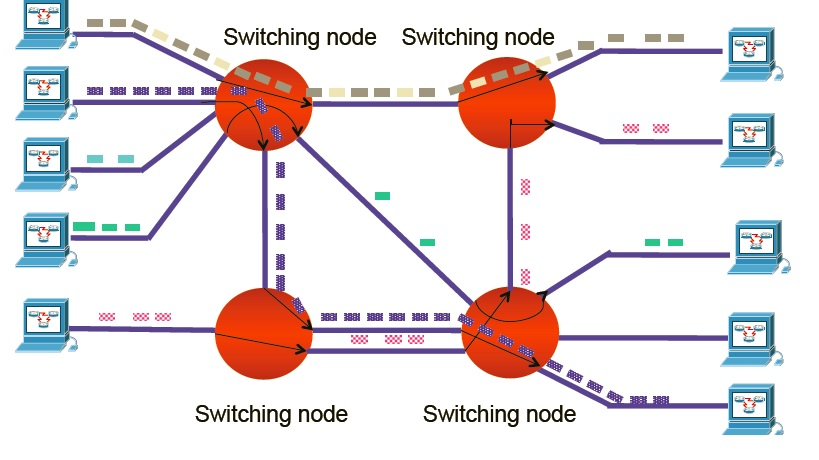
\includegraphics[width=0.8\textwidth]{CS.jpg}
\caption{\label{CS.jpg}Circuit Switching}
\end{figure}

\begin{itemize}
\item Are used for phone calls
\item Reserve a dedicated channel for the entire communication
\item Private Branch EXchange (PBX) system: First hardware for a circuit-switched network 
\item \textsc{Working Operation:} 
\begin{equation}
\begin{cases}
\bullet \text{ Electronic signals pass through several switches before a connec-}\\ \text{ -tion is established}\\
\bullet \text{\textbf{ During a call, no other network traffic can use those}} \\ \text{\textbf{ switches.}}
\end{cases}
\end{equation}
\end{itemize}

\subsubsection{Virtual Switching}

\subsubsection{Packet Switching}
\begin{equation}
\begin{cases}
\bullet \text{ Packet-switched networks move data in packets based on the}\\ \text{ destination address in each packet} \\
\bullet \text{ When received, packers are reassembled in the proper sequence} \\ \text{ to make up the original message}\\
\bullet \text{ Shared Resources} \rightarrow \text{Best Effort}
\end{cases}
\end{equation}

It consists in two basic operations:
\begin{equation}
\begin{cases}
\bullet \text{\textit{ \textbf{Routing}}}\\ \rotatebox[origin=c]{180}{$\Lsh$} \text{ Selection of the next hop}\\ \rotatebox[origin=c]{180}{$\Lsh$} \text{ Insertion of the IU in the buffer of the corrisponding output port}\\
\rotatebox[origin=c]{180}{$\Lsh$} \text{ Performed via software to allow for update of routing algorithms}\\
\bullet \text{ \textit{\textbf{Forwarding}}}\\ \rotatebox[origin=c]{180}{$\Lsh$} \text{ Physical transmission of the IU to the next hop}
\\ \rotatebox[origin=c]{180}{$\Lsh$} \text{ Is a \textit{hardware} operation}
\end{cases}
\end{equation}
The fact that the \textbf{forwarding} is a \textit{hardware} operation is due to \textbf{predetermination of the transmission techniques} $\rightarrow$ If a better transmission technique is available you just update the \textit{Network Interface Card (NIC)} of your switch $\rightarrow$ No need to change the routing software.

\subparagraph{PS-Networks}
\begin{figure}
\centering
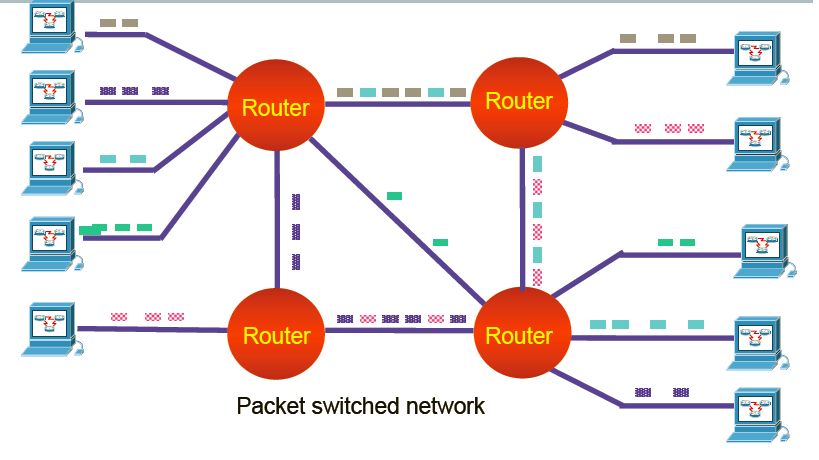
\includegraphics[width=0.8\textwidth]{PS.png}
\caption{\label{PS.png}Packet switching}
\end{figure}
\begin{itemize}
\item Are used to handle data
\item Power Computer Servers
\item \textsc{Working Operation:} 
\begin{equation}
\begin{cases}
\bullet \text{ The message gets broken into small data packets that seek out} \\ \text{ the most efficient route as circuits become available}\\
\bullet \text{ Each packet may go a different route.}\\
\bullet \text{ Its \textbf{header address tells it where to go and describes}} \\ \text{the sequence for reassembly at the destination compute.}\\
\bullet \text{ Packets arrival} \rightarrow \text{Queue of packets} \rightarrow \text{Statistical Multiplexing}
\end{cases}
\end{equation}
\end{itemize}
 
 
\subparagraph{Buffering}
\begin{figure}
\centering
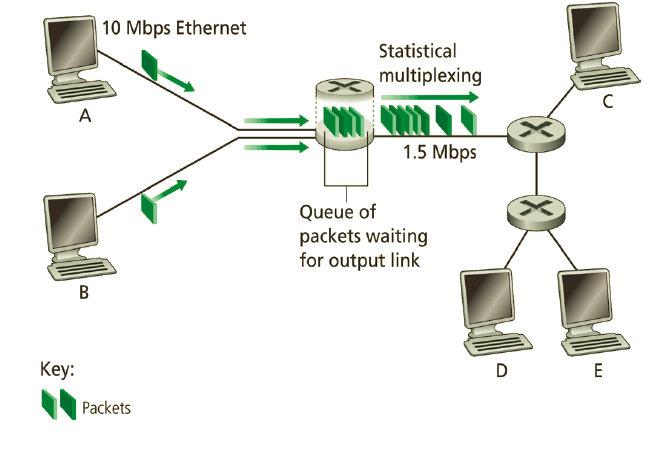
\includegraphics[width=0.8\textwidth]{PSBuffering.png}
\caption{\label{PSBuffering.png}Buffering in a PS Network}
\end{figure}


\subsection{Protocols}
\begin{definition}{\textbf{Protocol}\\}
A protocol is a set of rules that specify interactions between the communicating entities. We can say it is a language talked by \textsc{peer entities} of different devices.
\end{definition}
\begin{definition}{\textbf{Layer}\\}
A layer is a entity that offer services to its upper entity using the services offered by its lower layer entities.
\end{definition}
\begin{definition}{\textbf{Interface}\\}
An interface can be seen as a language talked by \textsc{neighbor} entities of the same device.
\end{definition}
\begin{definition}{\textbf{Embedding}\\}
Embedding is a concept which we refer to when considering the \textsc{Protocol Data Unit (PDU)} of upper layer as the \textsc{Service Data Unit (SDU)} of lower layer.
\end{definition}

\subsubsection{OSI model}
\begin{equation}\text{Host Layers = }
\begin{cases}
\text{\textbf{7. Application}} \Rightarrow \text{\textsc{data}} \\ \rotatebox[origin=c]{180}{$\Lsh$} \text{ Network Process to Application}\\
\text{\textbf{6. Presentation}} \Rightarrow \text{\textsc{data}}\\ \rotatebox[origin=c]{180}{$\Lsh$}
\text{ Data Representation and Encryption}\\
\text{\textbf{5. Session}} \Rightarrow \text{\textsc{data}}\\ \rotatebox[origin=c]{180}{$\Lsh$}
\text{ Inter-host Communications}\\
\text{\textbf{4. Transport}}\Rightarrow \text{\textsc{segments}}\\\rotatebox[origin=c]{180}{$\Lsh$} \text{ End-To-End Connections and Reliability}\\
\end{cases}\\
\end{equation}
\begin{equation}\text{Media Layers = }
\begin{cases}
\text{\textbf{3. Network}} \Rightarrow \text{\textsc{packets}}\\ \rotatebox[origin=c]{180}{$\Lsh$}
\text{Path Determination and IP} \rightarrow \text{Logical Addressing}\\
\text{\textbf{2. Data Link}} \Rightarrow \text{\textsc{frames}}\\ \rotatebox[origin=c]{180}{$\Lsh$}
\text{ MAC and LLC} \rightarrow \text{Physical addressing}\\
\text{\textbf{1. Physical}}\Rightarrow \text{\textsc{bits}}\\\rotatebox[origin=c]{180}{$\Lsh$} \text{ Media, Signal and Binary Transmission}
\end{cases}
\end{equation}

\begin{figure}
\centering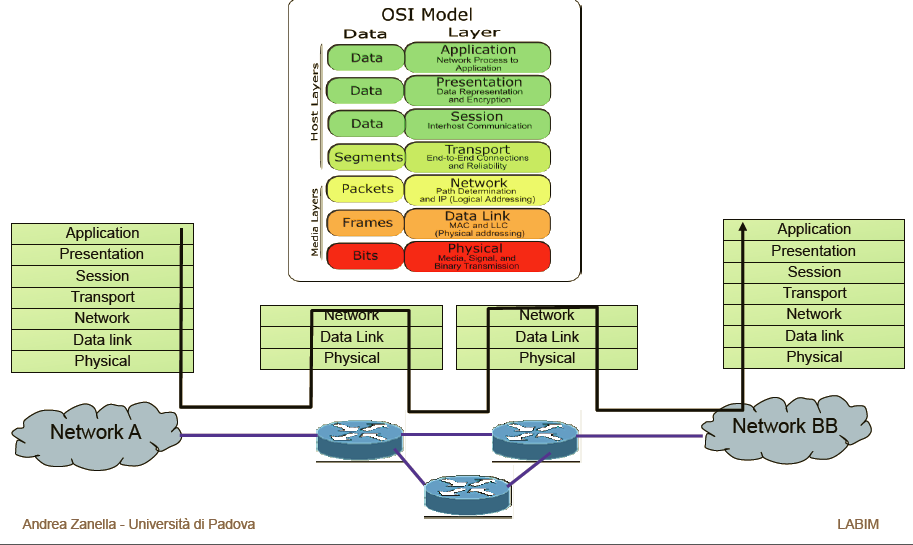
\includegraphics[width=0.8\textwidth]{OSImodel.png}
\caption{\label{OSImodel.png}Protocols accross network elements}
\end{figure}

\begin{figure}
\centering 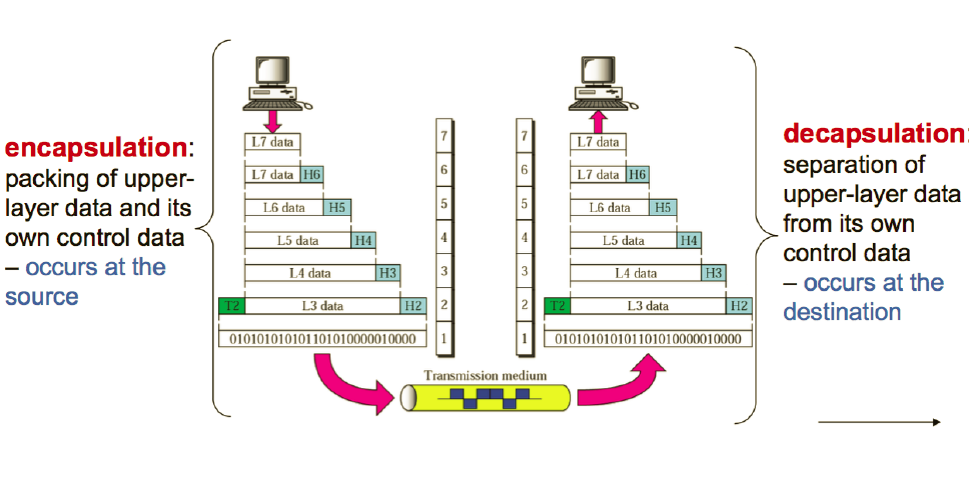
\includegraphics[width=0.9\textwidth]{ENCAPandDECAP.png}
\caption{\label{ENCAPandDECAP.png} Encapsulation and Decapsulation}
\end{figure}

\paragraph{OSI vs TCP/IP}
In the \textit{Internet Protocol Suite}, as we already have said, we have the two most important internet protocols (TCP and IP) and we can model every telecommunication system as the following TCP/IP protocol stack:
\begin{equation}\text{TCP/IP protocol stack = }
\begin{cases}
\text{\textbf{4. Application}} \\\rotatebox[origin=c]{180}{$\Lsh$} \text{ftp, telnet, smpt, http, x-windows}\\
\text{\textbf{3. Transport}} \\\rotatebox[origin=c]{180}{$\Lsh$} \text{TCP-UDP}\\
\text{\textbf{2. Internet}} \\\rotatebox[origin=c]{180}{$\Lsh$} \text{IP}\\
\text{\textbf{1. Subnet}} \\\rotatebox[origin=c]{180}{$\Lsh$} \text{Ethernet, Token-ring}
\end{cases}
\end{equation}

\paragraph{Request for Comments (RFC)}
A Request for Comments (RFC) is a type of publication from the \textit{Internet Engineering Task Force (IETF)} and the \textit{Internet Society (ISOC)}, the principal technical development and standards-setting bodies for the Internet. 

An RFC is authored by engineers and computer scientists in the form of a \textbf{memorandum describing methods}, \textbf{behaviors, research, or innovations applicable to the working of the Internet and Internet-connected systems}. It is submitted either for peer review or simply to convey new concepts, information, or (occasionally) engineering humor.[1] The IETF adopts some of the proposals published as RFCs as Internet Standards.

\subparagraph{Scheme}
This kind of items has to follow the follow scheme:

\begin{equation}\text{Internet Draft = }
\begin{cases}
\text{\textbf{1. Proposed Standard}}\\\rotatebox[origin=c]{180}{$\Lsh$} \text{\textit{1.1 Draft Standard}}\\
\rotatebox[origin=c]{180}{$\Lsh$}
\text{\textit{1.2 Internet Standard}} \\ \rotatebox[origin=c]{180}{$\Lsh$} \text{\textsc{Historic}}\\
\text{\textbf{2. Best Current Practice}} \\ \rotatebox[origin=c]{180}{$\Lsh$} \text{\textsc{Historic}}\\
\text{\textbf{3. Experimental}}\\ \rotatebox[origin=c]{180}{$\Lsh$} \text{\textsc{Historic}}\\
\text{\textbf{4. Informational}}\\ \rotatebox[origin=c]{180}{$\Lsh$} \text{\textsc{Historic}}         
\end{cases}
\end{equation}

\subparagraph{Requirements levels}
\begin{enumerate}
\item Required\\ $\rotatebox[origin=c]{180}{$\Lsh$}$ Must be implemented by all Internet systems (e.s IP and ICMP)
\item Recommended\\$\rotatebox[origin=c]{180}{$\Lsh$}$ Recommended but not required (e.s TCP)
\item Elective\\$\rotatebox[origin=c]{180}{$\Lsh$}$ Not required nor recommended, but feel free to use if you like
\item Limited use\\$\rotatebox[origin=c]{180}{$\Lsh$}$ Use in specific situations only (e.s experimental RFCs)
\item Not recommended\\$\rotatebox[origin=c]{180}{$\Lsh$}$ Not to be used 
\end{enumerate}

\subsection{Application architecture}
There are three types of application architecture:
\begin{enumerate}
	\item \textbf{Client-server}
	\begin{itemize}
	\item Server
		\begin{equation}
		\begin{cases}
		\text{ Always-on host}\\
        \text{ Permanent IP address}\\
		\text{ Server farms for scaling}
		\end{cases}
		\end{equation}
	\item Clients
		\begin{equation}
		\begin{cases}
		\text{ Communicate with server}\\
		\text{ May be intermittently connected}\\
		\text{ May have dynamic IP addresses}\\
		\text{\textbf{ Do not communicate directly with each other}}
		\end{cases}
		\end{equation}
	\end{itemize}
	\item \textbf{Peer-to-Peer (P2P)}\\ $\rotatebox[origin=c]{180}{$\Lsh$}$
\item \textbf{Hybrid of client-server and P2P}\\ $\rotatebox[origin=c]{180}{$\Lsh$}$
\end{enumerate}














% \input{chapter_2.tex}
% \input{chapter_PP.tex}
% \input{renewalProc.tex}
% \input{gbn_analysis.tex}
% \input{chapter_SN.tex}

\end{document}
